% !TeX spellcheck = sk_SK-Slovak
\documentclass[12pt, twoside]{book}
%\documentclass[12pt, oneside]{book}  % jednostranna tlac

%spravne nastavenie okrajov
\usepackage[a4paper,top=2.5cm,bottom=2.5cm,left=3.5cm,right=2cm]{geometry}
%zapnutie fontov pre UTF8 kodovanie
\usepackage[utf8]{inputenc}
\usepackage[T1]{fontenc}

%zapnutie slovenskeho delenia slov
%a automatickych nadpisov ako Obsah, Obrázok a pod. v slovencine
\usepackage[slovak]{babel} % vypnite pre prace v anglictine!

%nastavenie riadkovania podla smernice
\linespread{1.25} % hodnota 1.25 by mala zodpovedat 1.5 riadkovaniu

% balicek na vkladanie zdrojoveho kodu
\usepackage{listings}
% ukazky kodu su cislovane ako Listing 1,2,...
% tu je Listing zmenene na Algoritmus 1,2,...
\renewcommand{\lstlistingname}{Algoritmus}
% nastavenia balicka listings
% mozete pridat aj language=...
% na nastavenie najcastejsie pouzivaneho prog. jazyka
% takisto sa da zapnut cislovanie riadkov
\lstset{frame=lines}

% balicek na vkladanie obrazkov
\usepackage{graphicx}
% balicek na vkladanie celych pdf dokumentov, tu zadanie
\usepackage{pdfpages}
% balicek na spravne formatovanie URL
\usepackage{url}
% balicek na hyperlinky v ramci dokumentu
% zrusime farebne ramiky okolo liniek aby pdf
% vyzeralo rovnako ako tlacena verzia
\usepackage[hidelinks,breaklinks]{hyperref}

\usepackage{multirow}
\usepackage{cmap} 
%\usepackage{cm-super}

% -------------------
% --- Definicia zakladnych pojmov
% --- Vyplnte podla vasho zadania, rok ma byt rok odovzdania
% -------------------
\def\mfrok{2023}
\def\mfnazov{Získavanie štruktúrovaných dát \\o pacientoch s ochorením COVID-19 ~~~~~~~~~~z prepúšťacích správ a krvných výsledkov}
\def\mftyp{Bakalárska práca}
\def\mfautor{Marián Kravec}
\def\mfskolitel{Mgr. Vladimír Boža, PhD.}

%ak mate konzultanta, odkomentujte aj jeho meno na titulnom liste
\def\mfkonzultant{tit. Meno Priezvisko, tit. }  

\def\mfmiesto{Bratislava, \mfrok}

% študenti BIN a DAV odkomentujú príslušnú dvojicu riadkov
%\def\mfodbor{ Informatika}
%\def\program{ Informatika }
% pre BIN:
%\def\mfodbor{ Informatika a Biológia }
%\def\program{ Bioinformatika }
% pre DAV:
\def\mfodbor{ Informatika a Matematika } 
\def\program{ Dátová veda }

% Ak je školiteľ z FMFI, uvádzate katedru školiteľa, zrejme by mala byť aj na zadaní z AIS2
% Ak máte externého školiteľa, uvádzajte Katedru informatiky 
\def\mfpracovisko{ Katedra aplikovanej informatiky }

\begin{document}     
\frontmatter
\pagestyle{empty}

% -------------------
% --- Obalka ------
% -------------------

\begin{center}
\sc\large
Univerzita Komenského v Bratislave\\
Fakulta matematiky, fyziky a informatiky

\vfill

{\LARGE\mfnazov}\\
\mftyp
\end{center}

\vfill

{\sc\large 
\noindent \mfrok\\
\mfautor
}

\cleardoublepage
% --- koniec obalky ----

% -------------------
% --- Titulný list
% -------------------


\noindent

\begin{center}
\sc  
\large
Univerzita Komenského v Bratislave\\
Fakulta matematiky, fyziky a informatiky

\vfill

{\LARGE\mfnazov}\\
\mftyp
\end{center}

\vfill

\noindent
\begin{tabular}{ll}
Študijný program: & \program \\
Študijný odbor: & \mfodbor \\
Školiace pracovisko: & \mfpracovisko \\
Školiteľ: & \mfskolitel \\
% Konzultant: & \mfkonzultant \\
\end{tabular}

\vfill


\noindent \mfmiesto\\
\mfautor

\cleardoublepage
% --- Koniec titulnej strany


% -------------------
% --- Zadanie z AIS
% -------------------
% v tlačenej verzii s podpismi zainteresovaných osôb.
% v elektronickej verzii sa zverejňuje zadanie bez podpisov
% v pracach v angličtine anglické aj slovenské zadanie

\newpage 
\setcounter{page}{2}
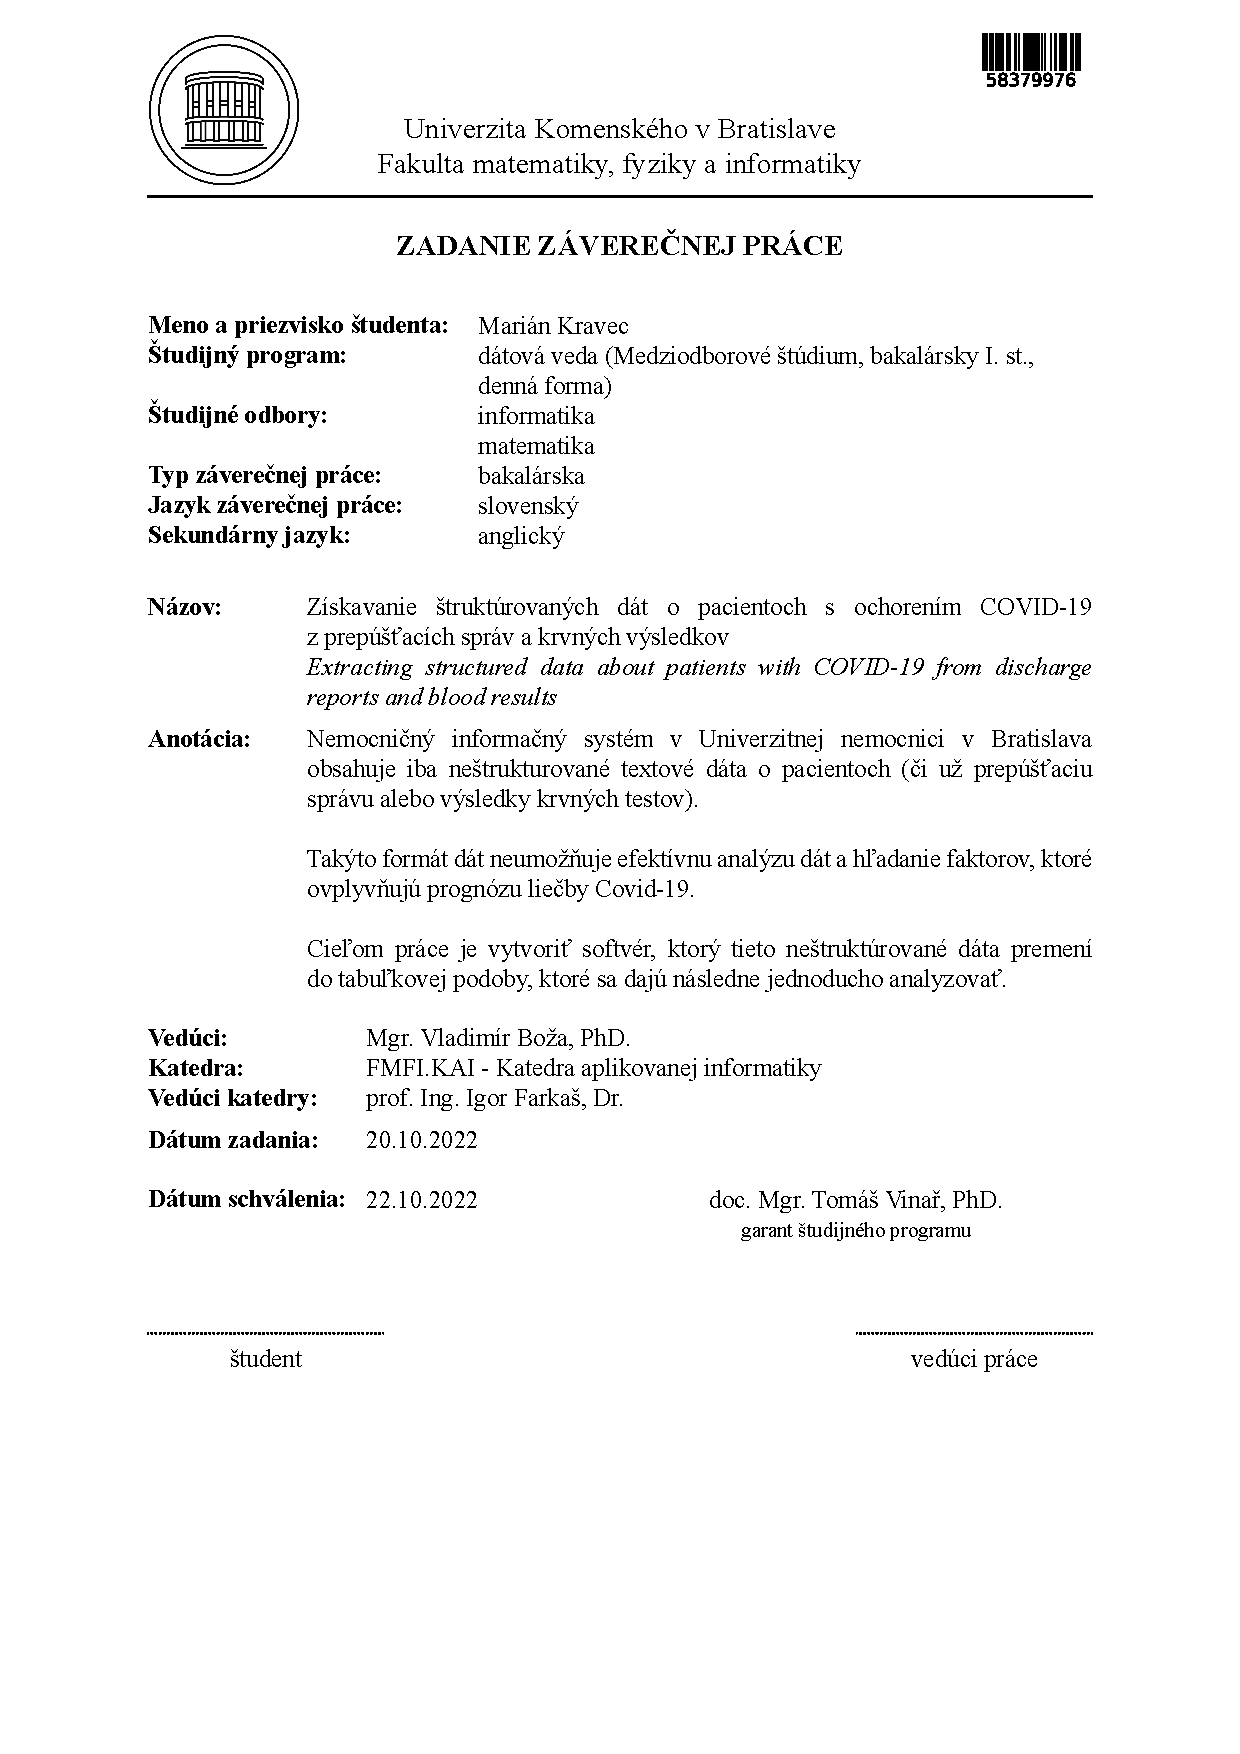
\includepdf{images/zadanie-zp_172972.pdf}
\newpage

\newpage
	
\newpage

\newpage
% --- Koniec zadania


% -------------------
%   Poďakovanie - nepovinné
% -------------------
\newpage 
\pagestyle{plain}
~

\vfill
{\bf Poďakovanie:} Touto cestou by som rád poďakoval svojmu školiteľovi Mgr. Vladimírovi Božovi, Phd. za ochotu a rady pri písaní práce a kódu. Zároveň by som rád poďakoval pánovi doc. MUDr. Petrovi Sabakovi, PhD. za umožnenie použitia kódu vyvinutého počas projektu na účely tejto práce.  

% --- Koniec poďakovania

% -------------------
%   Abstrakt - Slovensky
% -------------------
\newpage 
\section*{Abstrakt}


Nemocničný informačný systém v Univerzitnej nemocnici v Bratislava neumožňuje lekárovi získať štrukturalizované dáta o jednom pacientovi, respektíve o množine pacientov rýchlo a jednoducho, preto sme vytvorili systém ktorého úlohou je získavania požadovaných údajov z prepúšťacích správ a krvných výsledkov vďaka čomu sa práca lekára výrazne skrátila a zjednodušila. Systém je nastavený na získavanie informácii o pacientoch hospitalizovaných s ochorením COVID-19 z ich prepúšťacích správ a krvných výsledkov. Tento systém je však možné pomerne jednoducho upraviť pre získavanie inej množiny dát. Pri aktuálnom nastavení je náš systém výrazne rýchlejší a má porovnateľnú alebo nižšiu chybovosť ako ručné získavanie týchto dát.  

\paragraph*{Kľúčové slová:} prepúšťacia správa, regulárny výraz, získavanie dát
% --- Koniec Abstrakt - Slovensky


% -------------------
% --- Abstrakt - Anglicky 
% -------------------
\newpage 
\section*{Abstract}

Hospital information system in University Hospital in Bratislava does not allow the doctor to obtain structured data about one patient or a group of patients quickly and easily, therefore we have created a system whose task is to obtain the required informations from discharge reports and blood results, thanks to which the doctor's work has been significantly shortened and simplified. The system is set up for obtaining data on patients hospitalized with the disease of COVID-19 from their discharge reports and blood tests. However, this system can be modified relatively easily to retrieve a different set of data. With the current setup, our system is significantly faster and has a comparable or lower error rate than manual extraction of this data.


\paragraph*{Keywords:} discharge report, regular expresion, data extraction

% --- Koniec Abstrakt - Anglicky

% -------------------
% --- Predhovor - v informatike sa zvacsa nepouziva
% -------------------
%\newpage 
%
%\chapter*{Predhovor}
%
%Predhovor je všeobecná informácia o práci, obsahuje hlavnú charakteristiku práce 
%a okolnosti jej vzniku. Autor zdôvodní výber témy, stručne informuje o cieľoch 
%a význame práce, spomenie domáci a zahraničný kontext, komu je práca určená, 
%použité metódy, stav poznania; autor stručne charakterizuje svoj prístup a svoje 
%hľadisko. 
%
% --- Koniec Predhovor


% -------------------
% --- Obsah
% -------------------

\newpage 

\tableofcontents

% ---  Koniec Obsahu

% -------------------
% --- Zoznamy tabuliek, obrázkov - nepovinne
% -------------------

\newpage 

\listoffigures
%\listoftables

% ---  Koniec Zoznamov

\mainmatter
\pagestyle{headings}


\input uvod.tex 

%\input kapitola.tex

\input inePrace.tex

\input sprava.tex

%\input latex.tex

\input ziskavanie.tex

\input analyza.tex

\input modifikacie.tex

\input zaver.tex

% -------------------
% --- Bibliografia
% -------------------


\newpage	

\backmatter

\thispagestyle{empty}
\clearpage

\bibliographystyle{unsrt}
\bibliography{literatura} 


%---koniec Referencii

% -------------------
%--- Prilohy---
% -------------------

%Nepovinná časť prílohy obsahuje materiály, ktoré neboli zaradené priamo  do textu. Každá príloha sa začína na novej strane.
%Zoznam príloh je súčasťou obsahu.
%
\input appendixA.tex

%\input appendixB.tex

\end{document}






